\documentclass[11pt]{article}

\usepackage[a4paper,margin=2.2cm]{geometry}
\usepackage[T1]{fontenc}
\usepackage[utf8]{inputenc}
\usepackage{lmodern}
\usepackage{amsmath,amssymb,mathtools}
\usepackage{microtype}
\usepackage{enumitem}
\usepackage{titlesec}

\usepackage{tikz}
\usetikzlibrary{arrows.meta, calc}
\usepackage{float}
\usepackage[hidelinks]{hyperref}

\titleformat{\section}{\Large\bfseries}{\thesection}{0.75em}{}
\titleformat{\subsection}{\large\bfseries}{\thesubsection}{0.75em}{}
\titlespacing*{\section}{0pt}{1.4ex plus .2ex minus .2ex}{0.9ex}
\titlespacing*{\subsection}{0pt}{1.0ex plus .2ex minus .2ex}{0.5ex}

\newcommand{\R}{\mathbb{R}}
\newcommand{\adj}{\operatorname{adj}}
\newcommand{\diag}{\operatorname{diag}}

\begin{document}

\begin{center}
    {\LARGE\bfseries Dual-Gantry CT LPV-LFR Realization}\\[0.5em]
\end{center}

\vspace{0.7em}

\section{Introduction}

\begin{figure}[H]
\centering
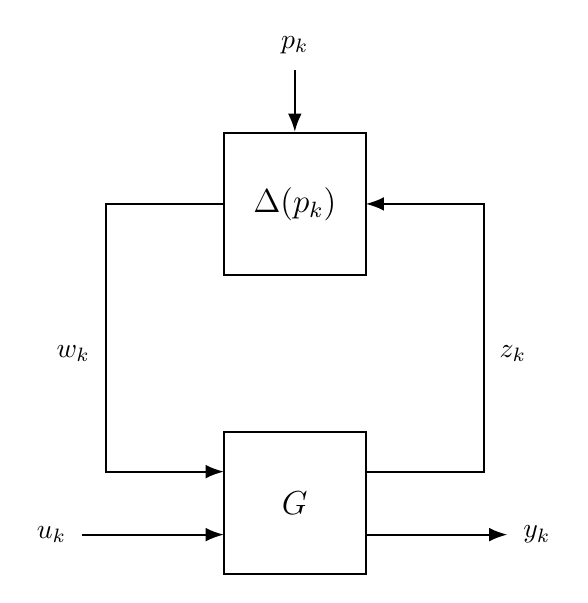
\begin{tikzpicture}[
  >=Latex,
  thick,
  block/.style={
    draw,
    rectangle,
    minimum width=1.8cm,
    minimum height=1.8cm,
    font=\large
  }
]

% --- Blocks ---
\node[block] (G)     at (0, 0)   {$G$};
\node[block] (Delta) at (0, 3.8) {$\Delta(p_k)$};

% --- Port vertical offset (upper/lower within G) ---
% G block half-height = 0.9; port offset from center:
\pgfmathsetmacro{\po}{0.4}   % port offset
\pgfmathsetmacro{\bw}{0.9}   % block half-width
\pgfmathsetmacro{\rx}{2.4}   % routing x distance from center

% --- p_k: top input into Delta ---
\draw[->] (0, 5.5) -- (Delta.north);
\node[above=2pt] at (0, 5.5) {$p_k$};

% --- w_k: Delta left → down left side → G upper-left ---
\draw[->]
  (-\bw, 3.8)          % Delta left port (center height)
  -- (-\rx, 3.8)        % go left
  -- (-\rx, \po)        % go down
  -- (-\bw, \po);       % enter G upper-left

\node[left=2pt] at (-\rx, 1.9) {$w_k$};

% --- z_k: G upper-right → up right side → Delta right ---
\draw[->]
  (\bw, \po)            % G upper-right port
  -- (\rx, \po)         % go right
  -- (\rx, 3.8)         % go up
  -- (\bw, 3.8);        % enter Delta right port

\node[right=2pt] at (\rx, 1.9) {$z_k$};

% --- u_k: external input into G lower-left ---
\draw[->] (-2.7, -\po) -- (-\bw, -\po);
\node[left=2pt] at (-2.7, -\po) {$u_k$};

% --- y_k: output from G lower-right ---
\draw[->] (\bw, -\po) -- (2.7, -\po);
\node[right=2pt] at (2.7, -\po) {$y_k$};

\end{tikzpicture}
\caption{Illustration of the interconnection between LPV plant and delta block in LFR representations.}
\label{fig:lpvlfr-structure}
\end{figure}
Figure~\ref{fig:lpvlfr-structure} shows the target LPV-LFR structure: the feedback interconnection between a constant LTI block $G$ and a scheduling block $\Delta(p_k)$. We derive a continuous-time LPV-LFR realization that exactly reproduces the
dual-gantry baseline model according to Drenth
\cite{drenth2025thesis}. The main construction step is to choose plant-specific latent variables and a repeated scheduling structure such that all scheduling dependence is contained in $\Delta$, while the state-space matrices of the LTI part $G$ remain constant. The realization is accepted only if eliminating the internal loop recovers the
original continuous-time state-space model exactly.


\section{Starting Point: Dual-Gantry CT Model}

The dual-gantry system is described in \emph{logical coordinates}
\[
q(t) = [X(t),\,\Theta(t),\,Y(t)]^\top \in \R^3,
\]
which are obtained from the physical stage positions $[X_1(t),\, X_2(t),\, Y(t)]^\top$ via the P-transform: $X = (X_1+X_2)/2$ (average lateral position), $\Theta = (X_1-X_2)/L_b$ (yaw angle), and $Y$ (tool-head lateral position). The equations of motion are
\begin{equation}
    M(Y)\,\ddot{q}(t) + C\,\dot{q}(t) + K\,q(t) = f_\ell(t),
    \label{eqs:eom}
\end{equation}
with
\begin{equation}
    M(Y) =
    \begin{bmatrix}
        m_1 + m_2 + m_b + m_h &
        \dfrac{(m_1-m_2)L_b}{2} - m_h Y &
        0 \\
        \dfrac{(m_1-m_2)L_b}{2} - m_h Y &
        J_b + J_h + \dfrac{(m_1+m_2)L_b^2}{4} + m_h d^2 + m_h Y^2 &
        -m_h d \\
        0 & -m_h d & m_h
    \end{bmatrix}.
    \label{eqs:mass}
\end{equation}
Here $C \in \R^{3\times3}$ and $K \in \R^{3\times3}$ denote the constant
viscous damping and stiffness matrices of the baseline gantry model. Note that $M(Y)$ has \emph{second-order polynomial} dependence in $Y$; the entries $-m_h Y$ and $m_h Y^2$ highlighted in \eqref{eqs:mass} make this explicit.
\\
The model is second order in $q(t)$, so we introduce the corresponding first-order
state vector
\begin{equation}
    x(t) = \begin{bmatrix} q(t) \\ \dot{q}(t) \end{bmatrix} \in \R^6.
    \label{eqs:state}
\end{equation}
Let
\begin{equation}
    u(t) := f_\ell(t)
    \label{eqs:input}
\end{equation}
denote the generalized input in logical coordinates. The MATLAB-derived
continuous-time state-space model is then
\begin{equation}
    \dot{x}(t) = A_c(Y)\,x(t) + B_c(Y)\,u(t),
    \qquad
    y(t) = C_c\,x(t),
    \label{eqs:ctss}
\end{equation}
with
\begin{equation}
    A_c(Y) =
    \begin{bmatrix}
        0 & I_3 \\
        -M(Y)^{-1}K & -M(Y)^{-1}C
    \end{bmatrix},
    \qquad
    B_c(Y) =
    \begin{bmatrix}
        0 \\
        M(Y)^{-1}
    \end{bmatrix},
    \qquad
    C_c = \begin{bmatrix} I_3 & 0 \end{bmatrix}.
    \label{eqs:ctmats}
\end{equation}
This is the model the LPV-LFR realization must recover after eliminating the internal loop.
\\
The output choice is
\begin{equation}
    y(t) = q(t).
    \label{eqs:yq}
\end{equation}
This matches the MATLAB model, because
\begin{equation}
    C_c\, x(t)
    =
    \begin{bmatrix} I_3 & 0 \end{bmatrix}
    \begin{bmatrix} q(t) \\ \dot{q}(t) \end{bmatrix}
    = q(t).
    \label{eqs:ccx}
\end{equation}

\section{Why the Dependence Is Rational}
The matrices in \eqref{eqs:ctmats} contain $M(Y)^{-1}$. Since $M(Y)$ is
polynomial in $Y$,
\begin{equation}
    M(Y)^{-1} = \frac{\adj(M(Y))}{\det(M(Y))},
    \label{eqs:adjdet}
\end{equation}
where $\adj(M(Y))$ and $\det(M(Y))$ are polynomial in $Y$, so the entries of
$M(Y)^{-1}$ are rational in $Y$. The ith element of the $i$-th row of $M(Y)^{-1}$ is therefore a rational function of $Y$. The continuous-time state-space model is therefore rational rather than affine
in $Y$. In Drenth's work, the LPV-LFR interconnection is ``equivalent to a
LPV-SS representation with rational dependency on $p(t)$'', while
``affine-dependency models are represented by taking (2.1) with $D_{zw}=0$''
\cite{drenth2025thesis}.

\section{Continuous-Time LPV-LFR Interconnection}
Drenth defines a continuous-time LPV-LFR as the interconnection between a
constant matrix $G$ and a scheduling block $\Delta(p)$
\cite{drenth2025thesis}. The equations are
\begin{align}
    \dot{x}(t) &= A_x x(t) + B_w w(t) + B_u u(t),
    \label{eqs:lfrstate} \\
    z(t) &= C_z x(t) + D_{zw} w(t) + D_{zu} u(t),
    \label{eqs:lfrz} \\
    y(t) &= C_y x(t) + D_{yw} w(t) + D_{yu} u(t),
    \label{eqs:lfry} \\
    w(t) &= \Delta(p(t)) z(t),
    \label{eqs:lfrw}
\end{align}
with constant matrix
\begin{equation}
    G =
    \begin{bmatrix}
        A_x & B_w & B_u \\
        C_z & D_{zw} & D_{zu} \\
        C_y & D_{yw} & D_{yu}
    \end{bmatrix}.
    \label{eqs:G}
\end{equation}
The matrices collected in $G$ are constant, so all scheduling dependence enters
through
\[
w(t)=\Delta(p(t))\,z(t).
\]
Drenth considers repeated block-diagonal scheduling structures of the form
\begin{equation}
    \Delta(p) =
    \diag\!\bigl(p_1 I_{\eta_1}, \dots, p_{n_p} I_{\eta_{n_p}}\bigr),
    \label{eqs:deltageneric}
\end{equation}
where $\eta_i$ is the number of repetitions of the scheduling variable $p_i$.


\section{Choice of Scheduling Variable}
The dual-gantry model has one physical scheduling variable, namely the logical
coordinate $Y$. Although powers of $Y$ appear in the model, they are not
introduced as separate independent scheduling variables. In line with Drenth's discussion of rational dependency
\cite{drenth2025thesis}, we retain the coupling between $Y$ and its powers by
reusing the same scheduling variable, rather than treating these terms as
independent scheduling variables.


\section{Latent Variables and Loop Signals}
Using the equations of motion \eqref{eqs:eom} and the state definition
\eqref{eqs:state}, the acceleration term satisfies
\begin{equation}
    M(Y)\,\ddot{q}(t)
    =
    -K q(t) - C\dot{q}(t) + u(t)
    =
    [-K\ {-C}]\,x(t) + u(t).
    \label{eqs:mechrewrite}
\end{equation}
Define the net force term
\begin{equation}
    f_{\mathrm{net}}(t) = [-K\ {-C}]\,x(t) + u(t).
    \label{eqs:fgen}
\end{equation}
Decompose the inertia matrix as
\begin{equation}
    M(Y) = M_0 + M_1 Y + M_2 Y^2,
    \label{eqs:decomp}
\end{equation}
with
\begin{align}
    M_0 &=
    \begin{bmatrix}
        m_1 + m_2 + m_b + m_h &
        \dfrac{(m_1-m_2)L_b}{2} &
        0 \\
        \dfrac{(m_1-m_2)L_b}{2} &
        J_b + J_h + \dfrac{(m_1+m_2)L_b^2}{4} + m_h d^2 &
        -m_h d \\
        0 & -m_h d & m_h
    \end{bmatrix},
    \label{eqs:M0} \\
    M_1 &=
    \begin{bmatrix}
        0 & -m_h & 0 \\
        -m_h & 0 & 0 \\
        0 & 0 & 0
    \end{bmatrix},
    \label{eqs:M1} \\
    M_2 &=
    \begin{bmatrix}
        0 & 0 & 0 \\
        0 & m_h & 0 \\
        0 & 0 & 0
    \end{bmatrix}.
    \label{eqs:M2}
\end{align}
Substituting \eqref{eqs:decomp} into \eqref{eqs:mechrewrite}:
\begin{equation}
    (M_0 + M_1 Y + M_2 Y^2)\,\ddot{q}(t) = f_{\mathrm{net}}(t).
    \label{eqs:polyexpand_M}
\end{equation}
Expanding the left-hand side:
\begin{equation}
    M_0\,\ddot{q}(t) + M_1\bigl(Y\ddot{q}(t)\bigr) + M_2\bigl(Y^2\ddot{q}(t)\bigr) = f_{\mathrm{net}}(t).
    \label{eqs:polyexpanded}
\end{equation}
The non-constant signal factors in \eqref{eqs:polyexpanded} are $Y\ddot{q}(t)$
and $Y^2\ddot{q}(t)$. Define the first latent variable
\begin{equation}
    z_1(t) := \ddot{q}(t) =
    \begin{bmatrix}
        \ddot{X}(t) \\
        \ddot{\Theta}(t) \\
        \ddot{Y}(t)
    \end{bmatrix} \in \R^3,
    \label{eqs:z1def}
\end{equation}
and introduce
\begin{equation}
    w_1(t) := Y\,z_1(t),
    \qquad
    z_2(t) := w_1(t),
    \qquad
    w_2(t) := Y\,z_2(t) = Y^2 z_1(t).
    \label{eqs:zwdefs}
\end{equation}
Since $Y$ is the only scheduling variable, $Y^2$ is realized by applying the same multiplier twice:
\begin{equation}
    z_1(t) \xrightarrow{\,Y\,} w_1(t) = z_2(t) \xrightarrow{\,Y\,} w_2(t),
    \label{eqs:Ychain}
\end{equation}
which corresponds to $\Delta(Y) = Y I_6$ applied once to $z(t) = [z_1(t);\, z_2(t)]$.
With these definitions, \eqref{eqs:polyexpanded} becomes
\begin{equation}
    M_0\,z_1(t) + M_1\,w_1(t) + M_2\,w_2(t) = f_{\mathrm{net}}(t).
    \label{eqs:constantrewrite}
\end{equation}
This turns the polynomial $Y$-dependence in \eqref{eqs:polyexpand_M} into a constant-matrix
relation, where $z_1(t)$, $z_2(t)$, $w_1(t)$, and $w_2(t)$ are derived latent vectors, not
additional physical states.

From \eqref{eqs:lfrw} and Figure~\ref{fig:lpvlfr-structure}, $w_1$ and $w_2$ must enter through $w$, so
\begin{equation}
    w(t) =
    \begin{bmatrix}
        w_1(t) \\
        w_2(t)
    \end{bmatrix}
    \in \R^6.
\end{equation}
Since $w(t) = \Delta(Y)z(t) = Y z(t)$, we need $z(t)$ such that $Yz(t) = [w_1(t),\, w_2(t)]^\top$.
From the chain \eqref{eqs:Ychain}, $Y z_1 = w_1$ and $Y z_2 = w_2$, so
\begin{equation}
    z(t) =
    \begin{bmatrix}
        z_1(t) \\
        z_2(t)
    \end{bmatrix}
    \in \R^6.
\end{equation}
Collecting both,
\begin{equation}
    z(t) =
    \begin{bmatrix}
        z_1(t) \\
        z_2(t)
    \end{bmatrix}
    \in \R^6,
    \qquad
    w(t) =
    \begin{bmatrix}
        w_1(t) \\
        w_2(t)
    \end{bmatrix}
    \in \R^6.
    \label{eqs:zw}
\end{equation}
To construct $\Delta(Y)$, we require $w(t) = \Delta(Y)z(t)$. From \eqref{eqs:Ychain},
\begin{equation}
    w(t) =
    \begin{bmatrix}
        w_1(t) \\
        w_2(t)
    \end{bmatrix}
    =
    \begin{bmatrix}
        Y z_1(t) \\
        Y z_2(t)
    \end{bmatrix}
    =
    \begin{bmatrix}
        Y I_3 & 0 \\
        0 & Y I_3
    \end{bmatrix}
    \begin{bmatrix}
        z_1(t) \\
        z_2(t)
    \end{bmatrix}
    =: \Delta(Y) z(t).
    \label{eqs:Deltaz}
\end{equation}
Hence
\begin{equation}
    \Delta(Y) =
    \begin{bmatrix}
        Y I_3 & 0 \\
        0 & Y I_3
    \end{bmatrix}
    = Y I_6.
    \label{eqs:Delta}
\end{equation}
Thus $\Delta(Y) = YI_6$ is one independent scheduler repeated over six latent
channels. This realization is not claimed to be minimal.


\section{Constant State-Space Matrices of the LTI Part $G$}
With the latent variables and loop signals fixed, it remains to find the
constant matrices of $G$. We rewrite the dual-gantry dynamics in terms of $x(t)$,
$w(t)$, and $u(t)$ following the block structure
\eqref{eqs:lfrstate}--\eqref{eqs:G}, and identify the entries of $A_x$, $B_w$, $B_u$,
$C_z$, $D_{zw}$, $D_{zu}$, $C_y$, $D_{yw}$, and $D_{yu}$.

\subsection{Expression for $z_1$}
From \eqref{eqs:constantrewrite}, solving for $z_1(t)$ with $M_0$ invertible:
\begin{equation}
    z_1(t) = M_0^{-1}[-K\ {-C}]\,x(t) - M_0^{-1}M_1\, w_1(t) - M_0^{-1}M_2\, w_2(t) + M_0^{-1}u(t).
    \label{eqs:z1expanded}
\end{equation}

\subsection{Derive the State Equation}
From \eqref{eqs:state} and \eqref{eqs:z1def},
\begin{equation}
    \dot{x}(t)
    =
    \begin{bmatrix}
        \dot{q}(t) \\
        z_1(t)
    \end{bmatrix}.
    \label{eqs:xdotz1}
\end{equation}
The upper block is
\begin{equation}
    \dot{q}(t)
    =
    \begin{bmatrix}
        0 & I_3
    \end{bmatrix}
    x(t),
    \label{eqs:qdotselector}
\end{equation}
because
\[
\begin{bmatrix}
    0 & I_3
\end{bmatrix}
\begin{bmatrix}
    q(t) \\
    \dot{q}(t)
\end{bmatrix}
= \dot{q}(t).
\]
For the lower block, note that
\begin{equation}
    M_0^{-1}[-K\ {-C}]
    =
    \begin{bmatrix}
        -M_0^{-1}K & -M_0^{-1}C
    \end{bmatrix}.
    \label{eqs:blocksplit}
\end{equation}
Substituting into \eqref{eqs:z1expanded},
\begin{equation}
    z_1(t)
    =
    \begin{bmatrix}
        -M_0^{-1}K & -M_0^{-1}C
    \end{bmatrix}
    x(t)
    +
    \begin{bmatrix}
        -M_0^{-1}M_1 & -M_0^{-1}M_2
    \end{bmatrix}
    w(t)
    +
    M_0^{-1}u(t).
    \label{eqs:z1finalblock}
\end{equation}
Stacking \eqref{eqs:qdotselector} and \eqref{eqs:z1finalblock} gives
\begin{equation}
    \dot{x}(t)
    =
    \begin{bmatrix}
        0 & I_3 \\
        -M_0^{-1}K & -M_0^{-1}C
    \end{bmatrix}
    x(t)
    +
    \begin{bmatrix}
        0 & 0 \\
        -M_0^{-1}M_1 & -M_0^{-1}M_2
    \end{bmatrix}
    w(t)
    +
    \begin{bmatrix}
        0 \\
        M_0^{-1}
    \end{bmatrix}
    u(t).
    \label{eqs:stateblocks}
\end{equation}
Therefore
\begin{equation}
    A_x =
    \begin{bmatrix}
        0 & I_3 \\
        -M_0^{-1}K & -M_0^{-1}C
    \end{bmatrix},
    \qquad
    B_w =
    \begin{bmatrix}
        0 & 0 \\
        -M_0^{-1}M_1 & -M_0^{-1}M_2
    \end{bmatrix},
    \qquad
    B_u =
    \begin{bmatrix}
        0 \\
        M_0^{-1}
    \end{bmatrix}.
    \label{eqs:ABmats}
\end{equation}

\subsection{Derive the Internal Output Equation}

From \eqref{eqs:zw}, $z(t) = [z_1(t);\, z_2(t)]$. The first block follows from
\eqref{eqs:z1finalblock}. For the second block, note from \eqref{eqs:zwdefs} that
$z_2(t) = w_1(t)$, which is the first half of $w(t)$ in \eqref{eqs:zw}:
\begin{equation}
    z_2(t) =
    \begin{bmatrix}
        I_3 & 0
    \end{bmatrix}
    w(t),
    \label{eqs:z2selector}
\end{equation}
with no dependence on $x(t)$ or $u(t)$. Stacking both blocks,
\begin{equation}
    z(t)
    =
    \begin{bmatrix}
        -M_0^{-1}K & -M_0^{-1}C \\
        0 & 0
    \end{bmatrix}
    x(t)
    +
    \begin{bmatrix}
        -M_0^{-1}M_1 & -M_0^{-1}M_2 \\
        I_3 & 0
    \end{bmatrix}
    w(t)
    +
    \begin{bmatrix}
        M_0^{-1} \\
        0
    \end{bmatrix}
    u(t),
    \label{eqs:loopblocks}
\end{equation}
so
\begin{equation}
    C_z =
    \begin{bmatrix}
        -M_0^{-1}K & -M_0^{-1}C \\
        0 & 0
    \end{bmatrix},
    \qquad
    D_{zw} =
    \begin{bmatrix}
        -M_0^{-1}M_1 & -M_0^{-1}M_2 \\
        I_3 & 0
    \end{bmatrix},
    \qquad
    D_{zu} =
    \begin{bmatrix}
        M_0^{-1} \\
        0
    \end{bmatrix}.
    \label{eqs:CDloop}
\end{equation}
\subsection{Derive the Output Equation}

The chosen output is $y(t)=q(t)$. Since
\[
x(t) =
\begin{bmatrix}
    q(t) \\
    \dot{q}(t)
\end{bmatrix},
\]
we have
\begin{equation}
    y(t) =
    \begin{bmatrix}
        I_3 & 0
    \end{bmatrix}
    x(t).
    \label{eqs:yfromx}
\end{equation}
There is no direct dependence on $w(t)$ or $u(t)$, so
\begin{equation}
    C_y =
    \begin{bmatrix}
        I_3 & 0
    \end{bmatrix},
    \qquad
    D_{yw} = 0,
    \qquad
    D_{yu} = 0.
    \label{eqs:Cy}
\end{equation}
The matrices \eqref{eqs:ABmats}, \eqref{eqs:CDloop}, and \eqref{eqs:Cy} define
the constant state-space matrix $G$ in \eqref{eqs:G}. The rows of $G$ correspond to $(\dot{x}, z, y)$ and the columns to $(x, w, u)$,
with dimensions $(6, 6, 3)$ in both cases, so
\[
G \in \R^{(6+6+3)\times(6+6+3)} = \R^{15\times15}.
\]

\section{Collapse to the Original CT Model}

Substituting $w(t) = \Delta(Y)z(t) = Y z(t)$ eliminates the internal loop. Using
\eqref{eqs:loopblocks} and \eqref{eqs:fgen}, the first block of the loop
equation becomes
\begin{equation}
    M_0 z_1(t) + Y M_1 z_1(t) + Y^2 M_2 z_1(t) = f_{\mathrm{net}}(t),
    \label{eqs:collapsecollect}
\end{equation}
which by \eqref{eqs:decomp} reduces to
\begin{equation}
    M(Y)\,z_1(t) = f_{\mathrm{net}}(t).
    \label{eqs:collapseMY}
\end{equation}
Since $M(Y)$ is invertible (see Section~\ref{sec:wellposed}),
\begin{equation}
    z_1(t) = M(Y)^{-1} f_{\mathrm{net}}(t).
    \label{eqs:collapsevinv}
\end{equation}
Substituting into \eqref{eqs:xdotz1} with \eqref{eqs:fgen} gives
\begin{equation}
    \dot{x}(t)
    =
    \begin{bmatrix}
        0 & I_3 \\
        -M(Y)^{-1}K & -M(Y)^{-1}C
    \end{bmatrix}
    x(t)
    +
    \begin{bmatrix}
        0 \\
        M(Y)^{-1}
    \end{bmatrix}
    u(t),
    \label{eqs:recoverstate}
\end{equation}
and the output equation is unchanged from \eqref{eqs:Cy}. Comparing with
\eqref{eqs:ctmats},
\begin{equation}
    A_{\mathrm{coll}}(Y) = A_c(Y),
    \qquad
    B_{\mathrm{coll}}(Y) = B_c(Y),
    \qquad
    C_{\mathrm{coll}} = C_c,
    \label{eqs:collapsedequal}
\end{equation}
so the LPV-LFR collapses exactly to \eqref{eqs:ctss}--\eqref{eqs:ctmats}.

\section{Well-Posedness}
\label{sec:wellposed}
\subsection{Drenth's Well-Posedness Condition}
Drenth requires that
\begin{equation}
    I - D_{zw}\Delta(p(t))
    \quad \text{is nonsingular for all } p(t)\in P.
    \label{eqs:drenthcriterion}
\end{equation}
For the present realization with single scheduling variable $Y$, this becomes
\begin{equation}
    I - D_{zw}\Delta(Y)
    \quad \text{is nonsingular for all } Y.
    \label{eqs:presentcriterion}
\end{equation}
Substituting $w(t)=\Delta(Y)z(t)$ into \eqref{eqs:lfrz} gives
\begin{equation}
    (I - D_{zw}\Delta(Y))\,z(t) = C_z x(t) + D_{zu}u(t).
    \label{eqs:genericloop}
\end{equation}
For given values of $x(t)$, $u(t)$, and $Y$, \eqref{eqs:genericloop} is a square
linear system in $z(t)$. Hence nonsingularity of $I-D_{zw}\Delta(Y)$ is equivalent
to unique solvability of \eqref{eqs:genericloop}.


\subsection{Reduction of the Loop Equation}
Using \eqref{eqs:CDloop} and \eqref{eqs:Delta},
\begin{equation}
    D_{zw}\Delta(Y)
    =
    \begin{bmatrix}
        -Y M_0^{-1}M_1 & -Y M_0^{-1}M_2 \\
        Y I_3 & 0
    \end{bmatrix},
    \label{eqs:DzwDelta}
\end{equation}
and therefore
\begin{equation}
    I - D_{zw}\Delta(Y)
    =
    \begin{bmatrix}
        I_3 + Y M_0^{-1}M_1 & Y M_0^{-1}M_2 \\
        -Y I_3 & I_3
    \end{bmatrix}.
    \label{eqs:IDzwDelta}
\end{equation}
Also,
\begin{equation}
    C_z x(t) + D_{zu}u(t)
    =
    \begin{bmatrix}
        M_0^{-1}[-K\ {-C}]\,x(t) + M_0^{-1}u(t) \\
        0
    \end{bmatrix}.
    \label{eqs:rhsloop}
\end{equation}
Substituting \eqref{eqs:zw}, \eqref{eqs:IDzwDelta}, and \eqref{eqs:rhsloop}
into \eqref{eqs:genericloop} yields
\begin{equation}
    \begin{bmatrix}
        I_3 + Y M_0^{-1}M_1 & Y M_0^{-1}M_2 \\
        -Y I_3 & I_3
    \end{bmatrix}
    \begin{bmatrix}
        z_1(t) \\
        z_2(t)
    \end{bmatrix}
    =
    \begin{bmatrix}
        M_0^{-1}[-K\ {-C}]\,x(t) + M_0^{-1}u(t) \\
        0
    \end{bmatrix}.
    \label{eqs:blockloop}
\end{equation}
The two block equations are
\begin{align}
    z_1(t) + Y M_0^{-1}M_1 z_1(t) + Y M_0^{-1}M_2 z_2(t)
    &= M_0^{-1}[-K\ {-C}]\,x(t) + M_0^{-1}u(t),
    \label{eqs:block1} \\
    -Y z_1(t) + z_2(t) &= 0.
    \label{eqs:block2}
\end{align}
From \eqref{eqs:block2},
\begin{equation}
    z_2(t) = Y z_1(t),
    \label{eqs:z2Yz1}
\end{equation}
consistent with \eqref{eqs:zwdefs}. Substituting \eqref{eqs:z2Yz1} into \eqref{eqs:block1}:
\begin{equation}
    z_1(t) + Y M_0^{-1}M_1 z_1(t) + Y^2 M_0^{-1}M_2 z_1(t)
    = M_0^{-1}[-K\ {-C}]\,x(t) + M_0^{-1}u(t).
    \label{eqs:z1reduced1}
\end{equation}
Multiply by $M_0$:
\begin{equation}
    M_0 z_1(t) + Y M_1 z_1(t) + Y^2 M_2 z_1(t) = [-K\ {-C}]\,x(t) + u(t) = f_{\mathrm{net}}(t).
    \label{eqs:z1reduced2}
\end{equation}
So for the dual-gantry realization, the loop equation reduces to
\begin{equation}
    M(Y)\,z_1(t) = f_{\mathrm{net}}(t),
    \qquad
    z_2(t) = Y z_1(t),
    \label{eqs:finalreduction}
\end{equation}
which is exactly the original mechanical relation \eqref{eqs:mechrewrite}.

\subsection{Well-Posedness of the Internal Loop}
From \eqref{eqs:finalreduction}, the internal loop has a unique solution if and
only if $M(Y)\,z_1(t) = f_{\mathrm{net}}(t)$ has a unique solution in $z_1(t)$, which holds
if and only if $M(Y)$ is invertible. Once $z_1(t)$ is unique, $z(t)$ and $w(t)$ follow directly from \eqref{eqs:zw} and
\eqref{eqs:Deltaz}. The internal loop is therefore well posed if and only if
$M(Y)$ is invertible.


% \subsection{Global Well-Posedness and Relation to Drenth's Section 2.2}

% The companion note \texttt{LPV/supporting/derivations/M-invertibility.tex} proves, using Sylvester's
% criterion, that under positive masses, inertias, and geometric parameters,
% \begin{equation}
%     M(Y) \succ 0
%     \qquad
%     \forall\, Y \in \R.
%     \label{eqs:MYpd}
% \end{equation}
% Therefore $M(Y)$ is invertible for all real $Y$, and the chosen LPV-LFR
% realization is globally well posed in $Y$.

% Drenth's Section~2.2 provides a generic sufficient well-posedness theorem based
% on diagonal $\Delta(p)$, bounded scheduling, and a spectral-radius condition on
% $D_{zw}$ \cite{drenth2025thesis}. That theorem is not the proof route used
% here. The present argument uses the plant-specific exact reduction
% \eqref{eqs:finalreduction} together with the companion proof of invertibility of
% $M(Y)$.
\section{Conclusion}
We have derived an exact continuous-time LPV-LFR realization of the dual-gantry
baseline model using one scheduling variable $Y$ represented through
$\Delta(Y) = YI_6$. The realization collapses exactly to \eqref{eqs:ctss}--\eqref{eqs:ctmats}
and is well posed if and only if $M(Y)$ is invertible. The LPV-LFR framework
and block-diagonal structure of $\Delta(p)$ follow Drenth \cite{drenth2025thesis};
the latent-variable construction and well-posedness reduction are plant-specific.
The realization is not claimed to be minimal.

\newpage
\begin{thebibliography}{9}

\bibitem{garcia2013model}
I.~Garc{\'i}a-Herreros, X.~Kestelyn, J.~Gomand, R.~Coleman, and P.-J.~Barre,
``Model-based decoupling control method for dual-drive gantry stages:
A case study with experimental validations,''
\textit{Control Engineering Practice}, vol.~21, no.~3, pp.~298--307, 2013.
doi: 10.1016/j.conengprac.2012.10.010.

\bibitem{drenth2025thesis}
R.~Drenth,
``Efficient Gradient-Based Learning of {LPV} Models with Linear Fractional Representation,''
M.Sc.\ thesis, Eindhoven University of Technology, Sept.\ 2025.

\end{thebibliography}

\end{document}
